\documentclass{article}
\usepackage[margin=1.2in]{geometry}
\usepackage{datetime}
%\usepackage{hyperref}      %for \url macro
\usepackage{microtype}     %attempt to fix issue with justification protrusion (in references)
\usepackage{amssymb}       % for formatting less/greater than symbols
\usepackage{amsmath}
\usepackage{enumitem}      %for changing spacing in bulleted lists
\usepackage{subfigure}        %for subfigures


\renewcommand{\arraystretch}{1.25}

\usepackage[gobble=auto, runall=true]{pythontex}
\usepackage{float} %for forcing position of images

\usepackage{graphicx}
\graphicspath{ {../images/} }
\usepackage[export]{adjustbox}
\usepackage[justification=centering]{caption}

\usepackage{listings}   %for typesetting code
\usepackage{color}
\definecolor{codegreen}{rgb}{0,0.6,0}
\definecolor{codegray}{rgb}{0.5,0.5,0.5}
\definecolor{codepurple}{rgb}{0.58,0,0.82}
\definecolor{backcolour}{rgb}{0.95,0.95,0.92}
\lstdefinestyle{mystyle}{
    backgroundcolor=\color{backcolour},
    commentstyle=\color{codegreen},
    keywordstyle=\color{codepurple},
    numberstyle=\tiny\color{codegray},
    stringstyle=\color{codepurple},
    basicstyle=\footnotesize,
    breakatwhitespace=false,
    breaklines=true,
    captionpos=b,
    keepspaces=true,
    %numbers=left,
    numbersep=5pt,
    showspaces=false,
    showstringspaces=false,
    showtabs=false,
    tabsize=2
}
\lstset{style=mystyle}

\frenchspacing                   %removes extra spacing after a period at the end of a sentence.
\newdateformat{daymonthyear}{\THEDAY\ \monthname\ \THEYEAR}

\title{CSC411 Machine Learning \\ Project 3: Fake News}
\author{ Ariel Kelman \\ Student No: 1000561368
         \\ \\
         Gideon Blinick \\ Student No: 999763000 }
\daymonthyear



\begin{document}
   \maketitle{}


   \section{Dataset Description}

Both datasets (real and fake) contain headlines about U.S. President Donald Trump.
From the headlines, it is very much possible to determine with significant accuracy the percentage chance that a given headline
is fake or real based on the precense of absence of certain words in the headline.
For example, after performing some preliminary analyses on the headlines, we discovered that the following 3 words might be of particular use.
\begin{enumerate}
\item The word "donald" appears 42.05\% of the time in real headlines while appearing in only 17.55\% of fake headlines. This 24.5\% difference was by far the largest of any word.

\item The word "the" appears 27.9\% of the time in fake headlines while appearing in only 7.9\% of real headlines for a difference of 20.02\%.
\item The word "trumps" appears 11.1\% of the time in real headlines while appearing in only 0.3\% of fake headlines for a difference of 10.8\%.
\end{enumerate}



   %\subsection{Results \& Report Reproducibility}



   \section{Naive Bayes Implementation}




   \section{Predictive Factors}




   \section{Logistic Regression}



   \section{Logistic Regression vs. Naive Bayes}
   When forming a prediction on a headline, both Naive Bayes and Logistic Regression effectively compute
   \begin{equation*}
      \theta^T I = \theta_0 + \theta_1 I_1 + \theta_2 I_2 + ... + \theta_k I_k > thr
   \end{equation*}
   where $thr$ is a given threshold value; in this project $thr = 0.5$. In both cases, the $\theta$'s represent
   the paremeters that define the prediction model, while the $I$'s are a function of the input for which a
   prediction is produced.

   For logistic regression, each $I = I(x)$ for a headline is simply a vector of $0$'s and $1$'s, where each
   position in the vector represents a word that was included in the training set. A $1$ indicates that the
   word is found in the headline, while a $0$ indicates that one was not. As the headlines are relatively short
   in comparison to the total number of words, this vector is very sparse. The $\theta$'s represent how important
   a feature (the presence of a particular word) is to the final prediction ($\theta_0$ is a bias that can
   account for the priors on real vs. fake headlines).

   For naive bayes,



   \section{Analysis of Logistic Regression}



   \section{Decision Tree}
   \subsection{Classification}
   Using the \texttt{sklearn} implementation of decision trees, we trained several decision trees
   to differentiate between the fake and real headlines. After some experimentation with the many parameters
   in the \texttt{sklearn DecisionTreeClassifier} (particularly with the maximum number of features used
   when looking for the best split), the default parameters gave the best results. As a split condition,
   maximum entropy was used rather than gini impurity, though similar results were obtained for both.
   Many of the settings served as ways to limit the size of the decision tree, so this result is not unexpected.

   Decision trees with a maximum depth of $\{ 2, 3, 5, 10, 15, 20, 35, 50, 75, 100, None \}$ were built, and
   the results on the training, validation, and testing sets are shown in the figure below. The final point,
   not plotted, with no limit on the maximum depth, gave an accuracy of $1, 0.76 0.76$ on the training,
   validation, and testing sets respectively.
      \begin{figure}[h] \centering

         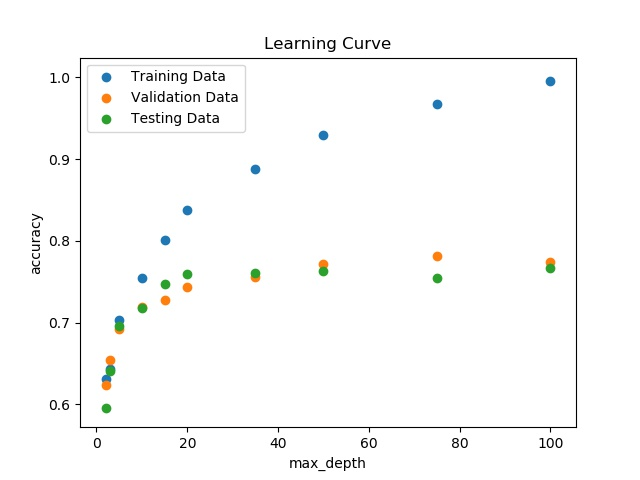
\includegraphics[width=4in]{resources/part7/part7a_splitCondition=entropy_maxFeatures=None_stopWords=True}

         \caption{Plot showing the preformance of \texttt{sklearn} decision trees with
            varying depth. The split condition was maximum entropy, there was no limit on the maximum
            number of features for a split, and stop words were included.}
      \end{figure}
   As can be seen from the figure, the larger the depth of the decision tree, the greater accuracy achieved on
   the testing set. However, improvement is small on the validation and testing sets after a depth of
   $~20$. Without any other constraints (such as a minimum number of samples to split a node), a decision tree
   can reach perfect accuracy on the training set, as demonstrated above. Predictably, this leads to
   much greater preformance on the training set than on the validation and testing sets (though there is no
   \textit{decrease} in preformance on the latter sets); showing the importance of using a validation and testing
   set to measure preformance.

   \subsection{Visualization}
   The following image shows the first few layers of the decision tree with depth $20$. It was generated by saving
   a text representation of the tree (as a \texttt{.dot} file), which was then visualized by using the
   %\texttt{webgraphviz} tool (available at \url{http://webgraphviz.com/}).
      \begin{figure}[h] \centering
       %  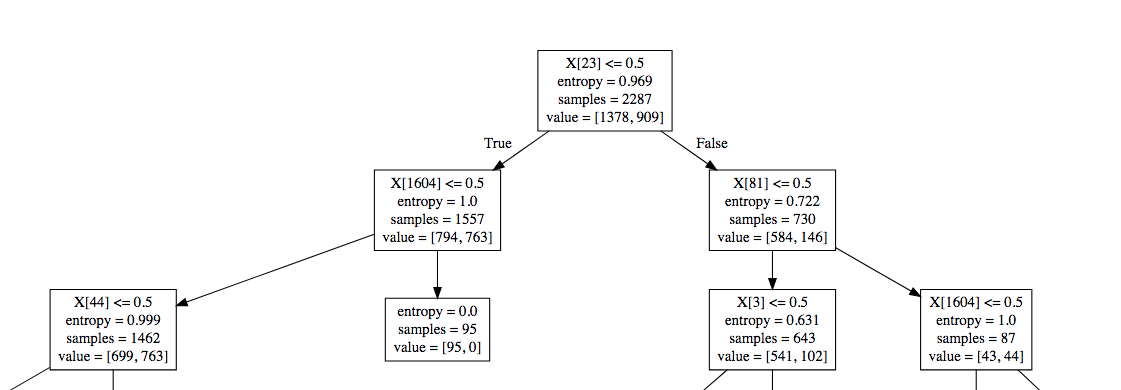
\includegraphics[width=4in]{resources/part7b}
         \caption{The top few layers of the decision tree (depth = 20).}
         \label{part7b}
      \end{figure}

   It is interesting to look at the words being split on in these layers; $X$ was a list of all words
   that appeared in either the fake or real datasets. These words are `donald' (23), `trumps' (1604; note the
   double appearance), `the' (81), `hillary' (44), and `trump' (3). The exact same process of training was run
   ignoring stop words, but results were slightly worse; graphs similar to those mentioned above can be found
   in the \texttt{resources} directory (each filename indicates whether stop words were included, as well as info
   on the other non-default parameters). Note that because of the use of dictionaries (i.e. because
   \texttt{dict.keys()} does not keep track of order), running the code again may result in different indices
   for each of the above words.


   A visualization of the entire tree is saves as \texttt{part7b_all.pdf}
   in the \texttt{resources} directory; the text represenations of many trees that were generated during
   training are saved in \texttt{resources/part7}.

   \subsection{Comparison of All 3 Classifiers}
   All three classifiers preform much better than random guessing...


   \section{Information Theory}
   \subsection{Mutual Information on First Split}
   Using the result from part 7, the word that produced the best initial split was `donald'. The mutual information
   (a measure of `information gain') on that split (on the training data) can be calculated by
   \begin{equation*} \begin{split}
      I(Y, x)  &= H(x) - H(x, Y) = H(Y) - H(Y,x)
   \end{split} \end{equation*}
   where $I$ is the mutual information, $H(x)$ is the entropy of $x$, and $H(x, Y)$ is the entropy of $x$ conditional
   on $Y$.
   Plugging in the values shown in Figure \ref{part7b} gives
   \begin{equation*} \begin{split}
      I(Y, x)  &= H(Y) - H(Y,x) \\
               &= 0.969 - \bigg[ P_1 (1) + P_2 (0.722)  \bigg] \\
               &= 0.969 - \bigg[ \frac{1557}{2287} (1) + \frac{730}{2287} (0.722)  \bigg] \\
               &= 0.0557
   \end{split} \end{equation*}
   where $x = `donald'$ and $Y$ indicates whether a headline is real or fake.

   A function \texttt{mutual_info()} was written to check this result, and to calculate the mutual
   information for other possible splits. The code for this function is shown below; it gave a result
   of 0.58 for $x = `donald'$.

      \begin{lstlisting}[language=Python]

         def mutual_info(word, y):
             count_word = 0 #number of headlines with word in training set
             lines_with_word = []
             lines_without_word = []
             for k in range(len(training_set)):
                 if word in training_set[k]:
                     count_word += 1
                     lines_with_word += [k]
                 else:
                     lines_without_word += [k]
             prob_word = count_word/len(training_set)

             y_with = np.array( [y[i] for i in lines_with_word] )
             y_without = np.array( [y[i] for i in lines_without_word] )

             prob_fake = np.count_nonzero(y)/len(y)
             H = prob_fake*np.log(prob_fake) + (1 - prob_fake)*np.log(1 - prob_fake) #entropy before split
             H = - H/np.log(2) #convert to base 2, and apply negative

             prob_fake_with = np.count_nonzero(y_with)/len(y_with)
             Hy = prob_fake_with*np.log(prob_fake_with) + (1 - prob_fake_with)*np.log(1 - prob_fake_with)
             Hy = - Hy/np.log(2) #entropy of headlines with word

             prob_fake_without = np.count_nonzero(y_without)/len(y_without)
             Hn = prob_fake_without*np.log(prob_fake_without) + (1 - prob_fake_without)*np.log(1 - prob_fake_without)
             Hn = - Hn/np.log(2)  #entropy of headlines without word

             I = H - (Hy*len(y_with) + Hn*len(y_without) )/len(y)
             return I
      \end{lstlisting}



   \subsection{Mutual Information on Later Split}
   The same procedure can be followed to compute the mutual information for a split on another word.
   Choosing a word randomly, gave a value of 0.0013 for the mutual information of a split of the training
   set on the word `ways'. As expected, this value is lower than the mutual information for a split on the
   word `donald' - that word was chosen as the first split precisely because it gave the most information
   about whether a headline was real or fake.



\end{document}
